% !TeX root = Report.tex
\section{Contiki Overview}

Contiki \cite{?} is on open source operating system for the internet of things, that we are using to power our WSN applications.

\subsection{Cooja}

Cooja \cite{?} is the simulator that we are using to test out algorithms on. One of the major benefits of using it is that the code written for the simulator is the same code that will be compiled for the wireless sensor nodes.

\subsection{Network Overview}

\begin{figure}[H]
	\centering
	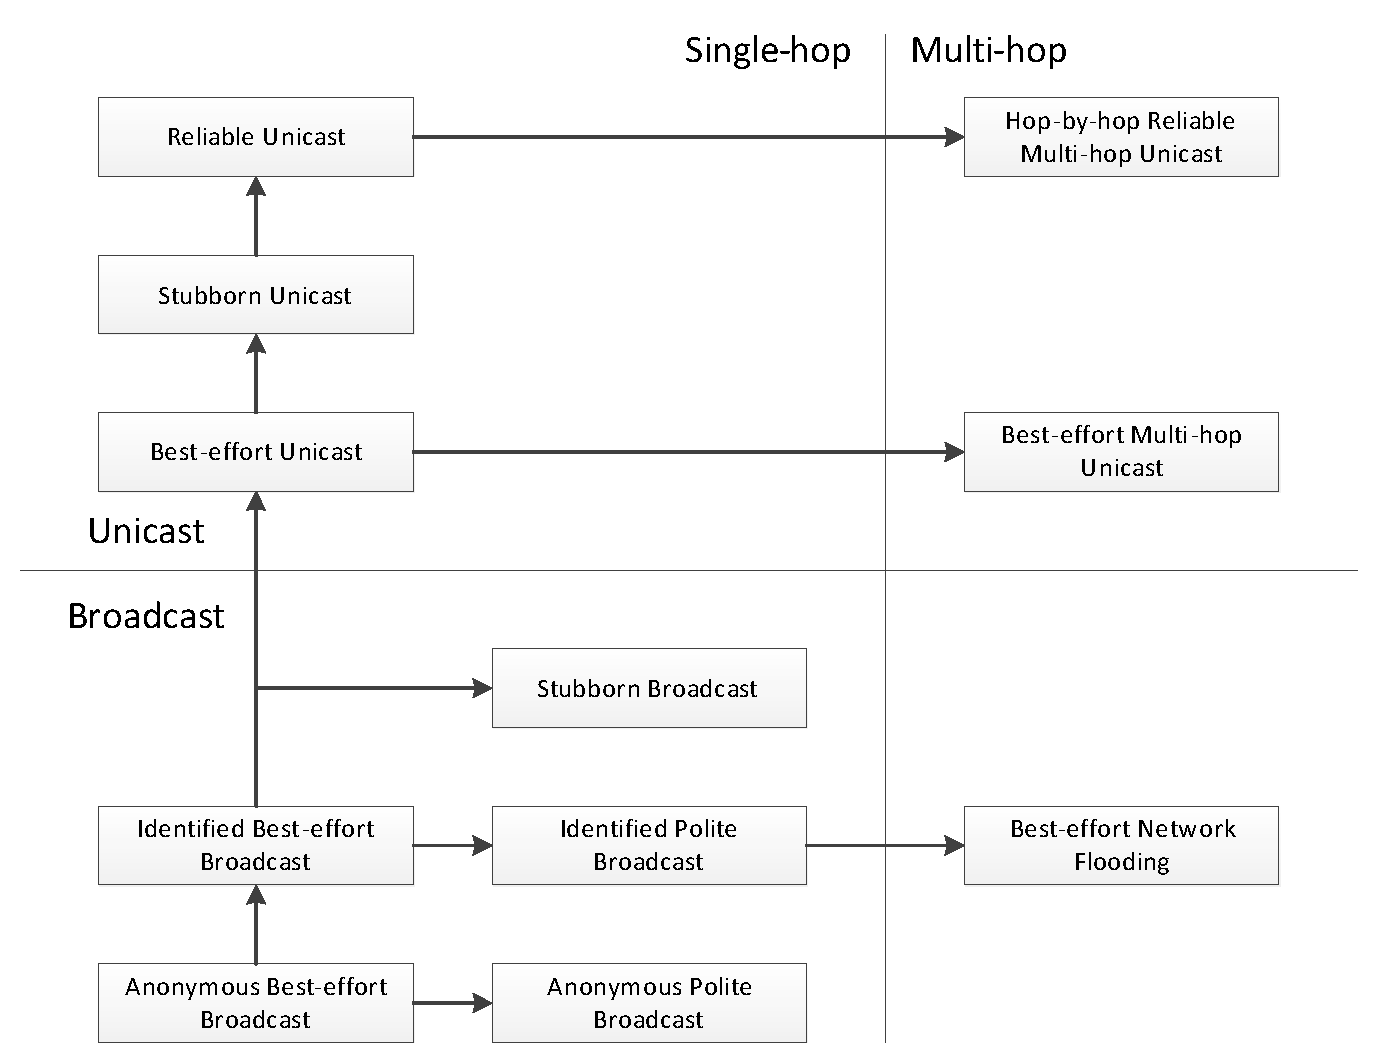
\includegraphics[width=\textwidth]{Diagrams/rime-stack}
	\caption{The communication primitives in the Rime network stack \cite{Dunkels:2007:ACA:1322263.1322295}}
\end{figure}

\begin{table}[H]
	\centering
	\begin{tabular}{ | l | l | l | }
		\hline
		Name & Header & Address \\
		\hline
		Anonymous Broadcast & abc.h & \url{contiki.sourceforge.net/docs/2.6/a01717.html} \\
		Broadcast & broadcast.h & \url{contiki.sourceforge.net/docs/2.6/a01720.html} \\
		Stubborn Broadcast & stbroadcast.h & \url{contiki.sourceforge.net/docs/2.6/a01739.html} \\
		Anonymous Polite Broadcast & polite.h & \url{contiki.sourceforge.net/docs/2.6/a01730.html} \\
		Polite Broadcast & ipolite.h & \url{contiki.sourceforge.net/docs/2.6/a01724.html} \\
		Unicast & unicast.h & \url{contiki.sourceforge.net/docs/2.6/a01738.html} \\
		Stubborn Unicast & stunicast.h & \url{contiki.sourceforge.net/docs/2.6/a01740.html} \\
		Reliable Unicast & runicast.h & \url{contiki.sourceforge.net/docs/2.6/a01738.html} \\
		Network Flooding & netflood.h & \url{contiki.sourceforge.net/docs/2.6/a01728.html} \\
		Multi-hop Unicast & multihop.h & \url{contiki.sourceforge.net/docs/2.6/a01726.html} \\
		Reliable Multi-hop Unicast & rmh.h & \url{contiki.sourceforge.net/docs/2.6/a01732.html} \\
		Reliable Unicast Bulk Transfer & rucb.h& \url{contiki.sourceforge.net/docs/2.6/a00365.html} \\
		\hline
		\hline
		Mesh & mesh.h & \url{contiki.sourceforge.net/docs/2.6/a01725.html} \\
		Collect & collect.h & \url{contiki.sourceforge.net/docs/2.6/a01723.html} \\
		Trickle & trickle.h & \url{contiki.sourceforge.net/docs/2.6/a01742.html} \\
		\hline
	\end{tabular}
	\caption{Communication Primitives headers and documentation location}
\end{table}


\begin{table}[H]
	\centering
	\begin{tabular}{ | l | l | l | l | }
		\hline
		Name & Reliable & Target & Sender Known\\
		\hline
		Anonymous Broadcast & No & 1-hop neighbours & No\\
		Broadcast & No & 1-hop neighbours & Yes\\
		Stubborn Broadcast & No & 1-hop neighbours & No\\
		Anonymous Polite Broadcast & No & 1-hop neighbours & No\\
		Polite Broadcast & No & 1-hop neighbours & Yes\\
		Unicast & No & destination & Yes\\
		Stubborn Unicast & No & destination & Yes\\
		Reliable Unicast & Yes & destination & Yes\\
		Network Flooding & No & network & Yes\\
		Multi-hop Unicast & No & destination & Yes\\
		Reliable Multi-hop Unicast & Yes & destination & Yes\\
		\hline
		\hline
		Mesh & No & destination & Yes \\
		Collect & Yes & destination & Yes \\
		Trickle & Yes & network & No \\
		\hline
	\end{tabular}
	\caption{Communication Primitives behaviour}
\end{table}

\subsubsection{Anonymous Best-effort Broadcast}

This is the most basic kind of message transmission primitive in Contiki's Rime network stack. It broadcasts a single packet with a maximum length to its 1-hop neighbours. No information about the sender is included within the transmission. It is not usually the case that this type of broadcast is used, as more reliable, more informative primitives (that are built on this one) are often used instead.

\begin{listing}[H]
\begin{minted}[fontsize=\small]{c}
void abc_open(struct abc_conn *c, uint16_t channel, const struct abc_callbacks *u);
void abc_close(struct abc_conn *c);
int abc_send(struct abc_conn *c);

struct abc_callbacks {
   void(* recv)(struct abc_conn *ptr);
};
\end{minted}
\caption{Contiki Anonymous Best-effort Broadcast APIs}
\end{listing}

\subsubsection{Identified Best-effort Broadcast}

This broadcast primitive is essentially the same as the Anonymous Best-effort Broadcast primitive, except for the fact that the address of the sender is included within the header of the message. This address is then made available to the developer when the \verb|recv| callback is called (as can been seen in \autoref{lst:IBEB}).

\begin{listing}[H]
\begin{minted}[fontsize=\small]{c}
void broadcast_open(struct broadcast_conn *c, uint16_t channel,
                    const struct broadcast_callbacks *u);
void broadcast_close(struct broadcast_conn *c);
int broadcast_send(struct broadcast_conn *c);

struct broadcast_callbacks {
   void(* recv)(struct broadcast_conn *ptr, const rimeaddr_t *sender);
};
\end{minted}
\caption{Contiki Identified Best-effort Broadcast APIs}
\label{lst:IBEB}
\end{listing}


\subsubsection{Stubborn Broadcast}

\begin{listing}[H]
\begin{minted}[fontsize=\small]{c}
void stbroadcast_open(struct stbroadcast_conn *c, uint16_t channel,
                      const struct stbroadcast_callbacks *u);
void stbroadcast_close(struct stbroadcast_conn *c);
void stbroadcast_set_timer(struct stbroadcast_conn *c, clock_time_t t);
int stbroadcast_send_stubborn(struct stbroadcast_conn *c, clock_time_t t);
void stbroadcast_cancel(struct stbroadcast_conn *c);

struct stbroadcast_callbacks {
   void (* recv)(struct stbroadcast_conn *c);
   void (* sent)(struct stbroadcast_conn *c);
};
\end{minted}
\caption{Contiki Stubborn Broadcast APIs}
\end{listing}

\subsubsection{Anonymous Polite Broadcast}

\begin{listing}[H]
\begin{minted}[fontsize=\small]{c}
void polite_open(struct polite_conn *c, uint16_t channel,
                 const struct polite_callbacks *cb);
void polite_close(struct polite_conn *c);
int polite_send(struct polite_conn *c, clock_time_t interval, uint8_t hdrsize);
void polite_cancel(struct polite_conn *c);

struct stbroadcast_callbacks {
   void(* recv)(struct polite_conn *c);
   void(* sent)(struct polite_conn *c);
   void(* dropped)(struct polite_conn *c);
};
\end{minted}
\caption{Contiki Anonymous Polite Broadcast APIs}
\end{listing}

\subsubsection{Identified Polite Broadcast}

\begin{listing}[H]
\begin{minted}[fontsize=\small]{c}
void ipolite_open(struct ipolite_conn *c, uint16_t channel,
                  uint8_t maxdups, const struct ipolite_callbacks *cb);
void ipolite_close(struct ipolite_conn *c);
int ipolite_send(struct ipolite_conn *c, clock_time_t interval, uint8_t hdrsize);
void ipolite_cancel(struct ipolite_conn *c);

struct stbroadcast_callbacks {
   void(* recv)(struct ipolite_conn *c, const rimeaddr_t *from)
   void(* sent)(struct ipolite_conn *c);
   void(* dropped)(struct ipolite_conn *c);
};
\end{minted}
\caption{Contiki Identified Polite Broadcast APIs}
\end{listing}

\subsubsection{Best-effort Unicast}

\begin{listing}[H]
\begin{minted}[fontsize=\small]{c}
void unicast_open(struct unicast_conn *c, uint16_t channel, const struct unicast_callbacks *u);
void unicast_close(struct unicast_conn *c);
int unicast_send(struct unicast_conn *c, const rimeaddr_t *receiver);

struct unicast_callbacks {
   void (* recv)(struct unicast_conn *c, const rimeaddr_t *from);
   void (* sent)(struct unicast_conn *ptr, int status, int num_tx);
};
\end{minted}
\caption{Contiki Best-effort Unicast APIs}
\end{listing}

\subsubsection{Stubborn Unicast}

\begin{listing}[H]
\begin{minted}[fontsize=\small]{c}
void stunicast_open(struct stunicast_conn *c, uint16_t channel,
                    const struct stunicast_callbacks *u);
void stunicast_close(struct stunicast_conn *c);
int stunicast_send_stubborn(struct stunicast_conn *c,
                            const rimeaddr_t *receiver, clock_time_t rxmittime);
void stunicast_cancel(struct stunicast_conn *c);
int stunicast_send(struct stunicast_conn *c, const rimeaddr_t *receiver);
void stunicast_set_timer(struct stunicast_conn *c, clock_time_t t);
rimeaddr_t *stunicast_receiver(struct stunicast_conn *c);

struct stunicast_callbacks {
   void (* recv)(struct stunicast_conn *c, const rimeaddr_t *from);
   void (* sent)(struct stunicast_conn *c, int status, int num_tx);
};
\end{minted}
\caption{Contiki Stubborn Unicast APIs}
\end{listing}

This is in fact anonymous, it will not send the address of the node that send the message in the header of the message. If a node needs to know who sent the message, then the sender's address should be included in the body.


\subsubsection{Reliable Unicast}

\begin{listing}[H]
\begin{minted}[fontsize=\small]{c}
void runicast_open(struct runicast_conn *c, uint16_t channel,
                   const struct runicast_callbacks *u);
int runicast_send(struct runicast_conn *c, const rimeaddr_t *receiver,
                  uint8_t max_retransmissions);
uint8_t runicast_is_transmitting(struct runicast_conn *c);

struct runicast_callbacks {
   void (* recv)(struct runicast_conn *c, const rimeaddr_t *from, uint8_t seqno);
   void (* sent)(struct runicast_conn *c, const rimeaddr_t *to, uint8_t retransmissions);
   void (* timedout)(struct runicast_conn *c, const rimeaddr_t *to, uint8_t retransmissions);
};
\end{minted}
\caption{Contiki Reliable Unicast APIs}
\end{listing}

\subsubsection{Best-effort Network Flooding}

\begin{listing}[H]
\begin{minted}[fontsize=\small]{c}
void netflood_open(struct netflood_conn *c, clock_time_t queue_time,
                   uint16_t channel, const struct netflood_callbacks *u);
void netflood_close(struct netflood_conn *c);
int netflood_send(struct netflood_conn *c, uint8_t seqno);

struct netflood_callbacks {
   int (* recv)(struct netflood_conn *c, const rimeaddr_t *from,
                const rimeaddr_t *originator, uint8_t seqno, uint8_t hops);
   void (* sent)(struct netflood_conn *c);
   void (* dropped)(struct netflood_conn *c);
};
\end{minted}
\caption{Contiki Best-effort Network Flooding APIs}
\end{listing}

\subsubsection{Best-effort Multi-hop Unicast}

\begin{listing}[H]
\begin{minted}[fontsize=\small]{c}
void rmh_open(struct rmh_conn *c, uint16_t channel, const struct rmh_callbacks *u);
void rmh_close(struct rmh_conn *c);
int rmh_send(struct rmh_conn *c, rimeaddr_t *to, uint8_t num_rexmit, uint8_t max_hops);

struct rmh_callbacks {
   void (* recv)(struct rmh_conn *ptr, rimeaddr_t *sender, uint8_t hops);
   rimeaddr_t *(* forward)(struct rmh_conn *ptr,
                          const rimeaddr_t *originator,
                          const rimeaddr_t *dest,
                          const rimeaddr_t *prevhop,
                          uint8_t hops);
};
\end{minted}
\caption{Contiki Best-effort Multi-hop Unicast APIs}
\end{listing}

\subsubsection{Hop-by-hop Reliable Multi-hop Unicast}

\begin{listing}[H]
\begin{minted}[fontsize=\small]{c}
void multihop_open(struct multihop_conn *c, uint16_t channel,
                   const struct multihop_callbacks *u);
void multihop_close(struct multihop_conn *c);
int multihop_send(struct multihop_conn *c, const rimeaddr_t *to);
void multihop_resend(struct multihop_conn *c, const rimeaddr_t *nexthop);

struct multihop_callbacks {
   void (* recv)(struct multihop_conn *ptr,
                 const rimeaddr_t *sender,
                 const rimeaddr_t *prevhop,
                 uint8_t hops);
   rimeaddr_t *(* forward)(struct multihop_conn *ptr,
                           const rimeaddr_t *originator,
                           const rimeaddr_t *dest,
                           const rimeaddr_t *prevhop,
                           uint8_t hops);
};
\end{minted}
\caption{Contiki Hop-by-hop Reliable Multi-hop Unicast APIs}
\end{listing}


\subsection{Mesh Network Protocol}

\begin{listing}[H]
\begin{minted}[fontsize=\small]{c}
void mesh_open(struct mesh_conn *c, uint16_t channels, const struct mesh_callbacks *callbacks);
void mesh_close(struct mesh_conn *c);
int mesh_send(struct mesh_conn *c, const rimeaddr_t *dest);

struct mesh_callbacks {
   /** Called when a packet is received. */
   void (* recv)(struct mesh_conn *c, const rimeaddr_t *from, uint8_t hops);
   /** Called when a packet, sent with mesh_send(), is actually transmitted. */
   void (* sent)(struct mesh_conn *c);
   /** Called when a packet, sent with mesh_send(), times out and is dropped. */
   void (* timedout)(struct mesh_conn *c);
};
\end{minted}
\caption{Contiki Mesh Network APIs}
\end{listing}


\subsection{Collect Network Protocol}

\begin{listing}[H]
\begin{minted}[fontsize=\small]{c}
void collect_open(struct collect_conn *c,
                  uint16_t channels, uint8_t is_router,
                  const struct collect_callbacks *callbacks);
void collect_close(struct collect_conn *c);
int collect_send(struct collect_conn *c, int rexmits);
void collect_set_sink(struct collect_conn *c, int should_be_sink);
int collect_depth(struct collect_conn *c);
const rimeaddr_t *collect_parent(struct collect_conn *c);
void collect_set_keepalive(struct collect_conn *c, clock_time_t period);

struct collect_callbacks {
   void (* recv)(const rimeaddr_t *originator, uint8_t seqno,
                 uint8_t hops);
};
\end{minted}
\caption{Contiki Collect Network APIs}
\end{listing}


\subsection{Trickle Network Protocol}

\begin{listing}[H]
\begin{minted}[fontsize=\small]{c}
void trickle_open(struct trickle_conn *c, clock_time_t interval,
                  uint16_t channel,
                  const struct trickle_callbacks *cb);
void trickle_close(struct trickle_conn *c);
void trickle_send(struct trickle_conn *c);

struct trickle_callbacks {
   void (* recv)(struct trickle_conn *c);
};
\end{minted}
\caption{Contiki Trickle Network APIs}
\end{listing}


\subsection{Network Channels}

Channels in Contiki are virtual \cite{tel-aviv-contiki-exercises, Dunkels:2007:ACA:1322263.1322295}. This means that when a connection is opened if you do not want to receive packets from another connection then a different channel should be used. It does not mean that different radio frequencies are used. To use different radio frequencies the function \verb|cc2420_set_channel| should be used to change the frequency messages are broadcasted on.


\subsection{Timers}

\subsubsection{Event Timer}

\url{http://contiki.sourceforge.net/docs/2.6/a01667.html}

\subsubsection{Callback Timer}

\url{http://contiki.sourceforge.net/docs/2.6/a01666.html}


\subsection{Optimisation}

\subsection{LTO and Whole Program}

Its is a shame that the developers of Contiki seem unwilling to support LTO (Link-Time Optimisations) that could greatly decrease the size of the binary and optimise the code \url{http://comments.gmane.org/gmane.comp.hardware.texas-instruments.msp430.gcc.user/11006}.

\subsection{Memory}

